\documentclass{article}

% Language setting
% Replace `english' with e.g. `spanish' to change the document language
\usepackage[english]{babel}

% Set page size and margins
% Replace `letterpaper' with`a4paper' for UK/EU standard size
\usepackage[letterpaper,top=2cm,bottom=2cm,left=3cm,right=3cm,marginparwidth=1.75cm]{geometry}


% Useful packages
\usepackage{amsmath}
\usepackage{graphicx}
\usepackage[colorlinks=true, allcolors=blue]{hyperref}
\usepackage{float}
\usepackage{caption}
\usepackage{subcaption}
%Path
\graphicspath{{figures/}}

\title{Personal Notes, Ideas, and Notes on Papers}
\author{Kristian Wold}

\begin{document}
\maketitle

\section{Personal Notes}

\subsection{Phase Fix of Observation}

In the reinforcement setting for quantum compiling, the environment is defined by the following objects

\begin{itemize}
    \item $U_T$, the target unitary to be compiled
    \item $U_n$ a sequence of $n$ elementary gates comping from a finite (presumably universal) set of gates
    \item $\epsilon$, a tolerance indicating how well $U_n$ should approximate $U_T$
\end{itemize}

The state of the environment, which the agent observes when deciding what elementary gate to include next, is given by

\begin{equation*}
    O_n = U_n U_T^{\dagger}
\end{equation*}
This matrix contains complete information about the "discrepancy" between the target unitary $U_T$ and the so-far compiled unitary $U_n$. In the case that $U_n$ approximates $U_T$, $O_n$ will approximate identity, up to a global phase.

The policy of the agent can be formulated as

\begin{equation*}
    \pi(O_n; \theta) = a_n \in [1,2, \cdots , m],
\end{equation*}
where $\pi$ is a neural policy parameterized by $\theta$, and $m$  is the number of elementary gates. After choosing an action, the environment updates as 

\begin{equation*}
    O_{n+1} = G_{a_{n}}O_{n}
\end{equation*}
\begin{equation*}
    U_{n+1} = G_{a_{n}}U_{n}
\end{equation*} 

For a given $O_n$, assume the best possible next elementary gate is $i$, and that the neural policy successfully identifies this gate. Since the action of operators are invariant under a global phase, $i$ should also be the best choice given $e^{i\phi}O_n$. However, the neural policy is not informed of this, and must explicitly learn the invarince of the global phase through training, which makes the learning problem potentially harder. This can be avoided by "fixing" the global phase of $O_n$ before sending it to the agent:

\begin{equation*}
    O_n \rightarrow e^{-i\gamma}O_n
\end{equation*}
where $\gamma = phase(O_n[0,0])$, i.e. the phase of the first element of $O_n$ in matrix representation. This fixates the global phase such that the first element of $O_n$ is always real. Thus, the neural policy is never exposed observations that differ in a global phase only, simplifying the learning problem.

\begin{figure}[H]
\begin{subfigure}{.5\textwidth} 
    \centering
    % include first image
    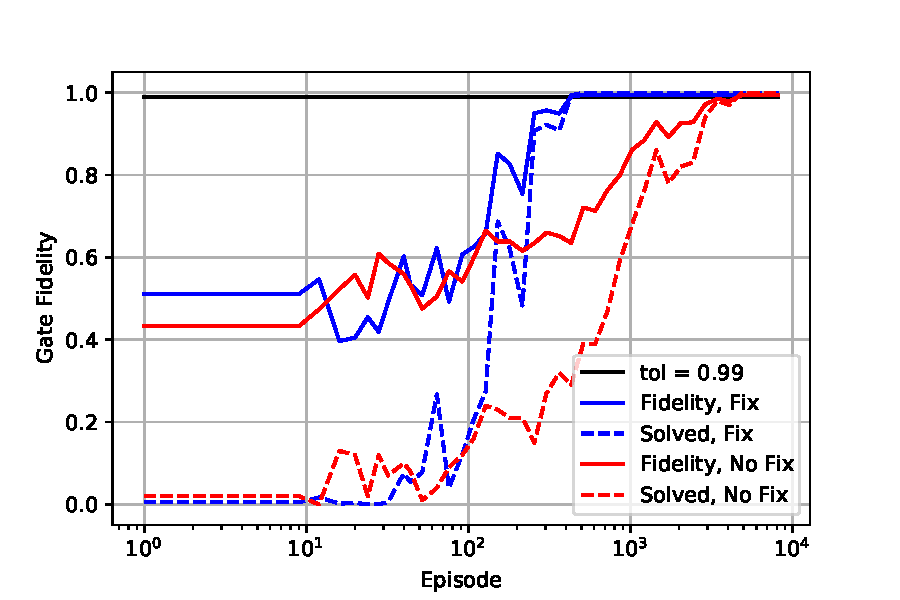
\includegraphics[width=.9\linewidth]{latex/figures/one_qubits_hrc_haarmeasure.pdf}  % this sets the image to fill 90% of the available space -> 45% of the line width in total. 
    \caption{One qubit, HRC}
    \label{fig:sub-first}
\end{subfigure}
\begin{subfigure}{.5\textwidth}
    \centering
    % include second image
    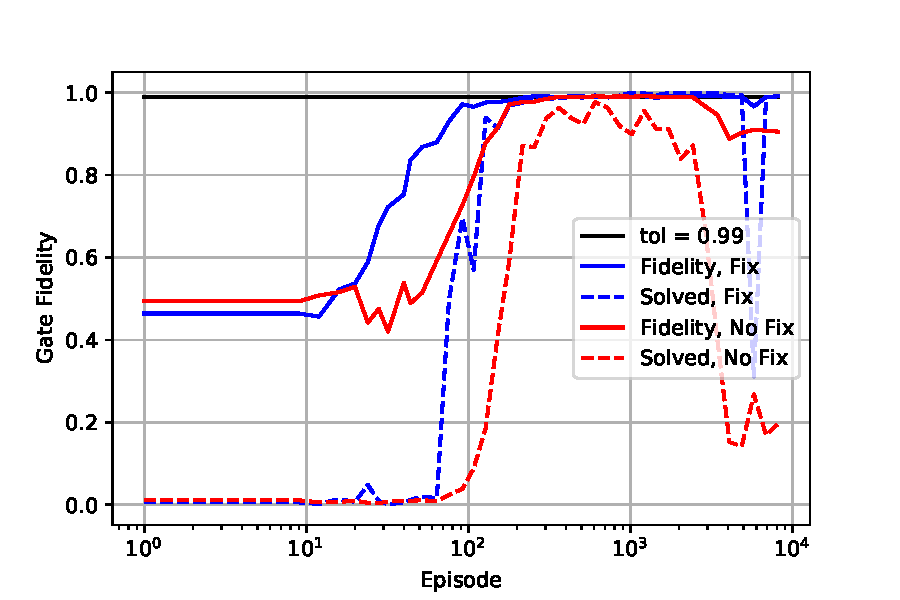
\includegraphics[width=.9\linewidth]{latex/figures/one_qubits_small_haarmeasure.pdf}  
    \caption{Two qubits, HRC}
    \label{fig:sub-second}
\end{subfigure}
\caption{HRC Basis on one, two and three qubits}
\label{fig:RL phase fix}
\end{figure}

As seen from the above figure, the phase fix greatly increase the training speed and stability of the training for both the HRC and Small Rotations for one qubit.

\subsection{Monte-Carlo Compiler with Metropolis}
Assume we have a finite set of elementary gates $\mathcal{B}$ and a target unitary $U_T$ that we want to approximate using a finite sequence of gates $U_n = G_1 G_2 \cdots G_n$ coming from this set, i.e. $G_i \in \mathcal{B}$. This sequence can be iteratively optimized in a Monte-Carlo fashion in the following way:

\begin{enumerate}
    \item Initiate a random sequence $U_{current}$ consisting of $n$ gates
    \item Calculate $fid_{current} = f(U_T, U_{current})$
    \item Create a new sequence $U_{new}$ by either inserting, removing or changing a random gate of $U_{current}$
    \item Recalculate the fidelity $fid_{new} = f(U_T, U_{new})$
    \item If $fid_{new} > fid_{current}$, the new sequence accepted. Otherwise, the change is rejected.
    \item repeat 3-5 until convergence or for a set amount
\end{enumerate}

The above algorithm is a very greedy search, performing only local changes and only keeping solutions that are strictly better. This makes it prone to getting stuck in local minima. To incentivize exploration, we can replace point 5 with a Metropolis-Hastings acceptance criterion:

\begin{enumerate}
    \item Calculate the amplitude $amp = e^{(fid_{new} - fid_{current})/T}$
    \item Sample a uniform variable $u \sim U[0,1]$
    \item Accept new sequence if $amp > u$
\end{enumerate}

Using the Metropolis-Hastings criterion, the optimizer will always accept better solutions, but will also sometimes accept worse solutions. This can be useful for getting out of local minima. By changing the temperature parameter $T$, one can tune how often worse solutions should be accepted. In the limit $T \rightarrow 0$, the acceptance criterion converges to the greedy criterion.

\subsubsection*{Results, Metropolis + Static T}
\begin{figure}[H]

\begin{subfigure}{.5\textwidth} 
    \centering
    % include first image
    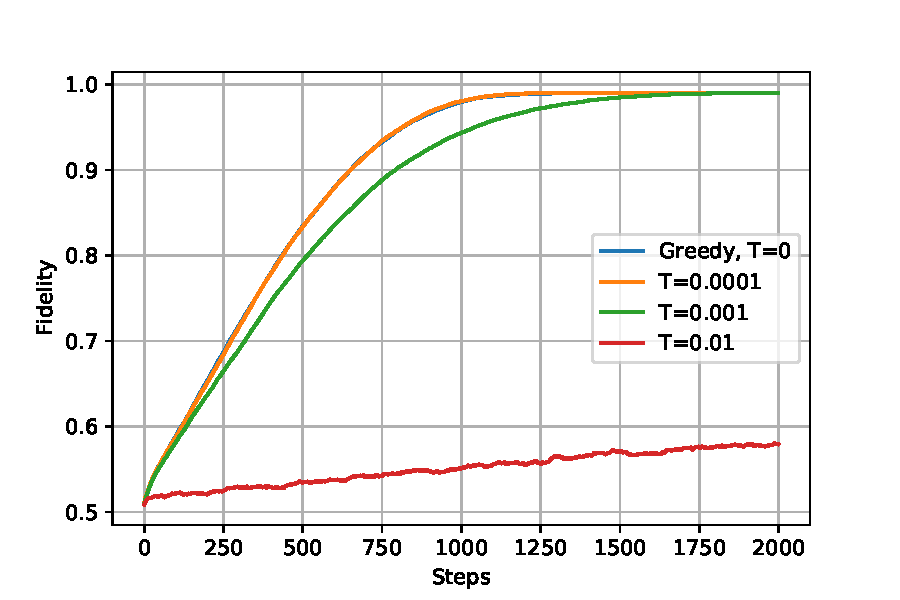
\includegraphics[width=.9\linewidth]{latex/figures/mcc_one_qubit_smallRot.pdf}  % this sets the image to fill 90% of the available space -> 45% of the line width in total. 
    \caption{One qubit, small rotations}
    \label{fig:sub-first}
\end{subfigure}
\begin{subfigure}{.5\textwidth}
    \centering
    % include second image
    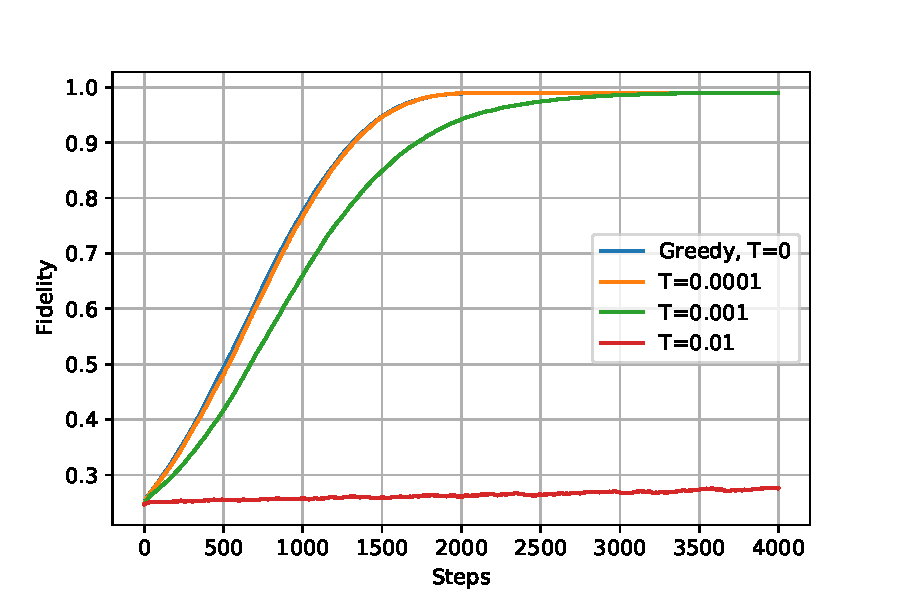
\includegraphics[width=.9\linewidth]{latex/figures/mcc_two_qubit_smallRot.pdf}  
    \caption{Two qubits, small rotations}
    \label{fig:sub-second}
\end{subfigure}


\begin{subfigure}{\textwidth}
    \centering
    % include first image
    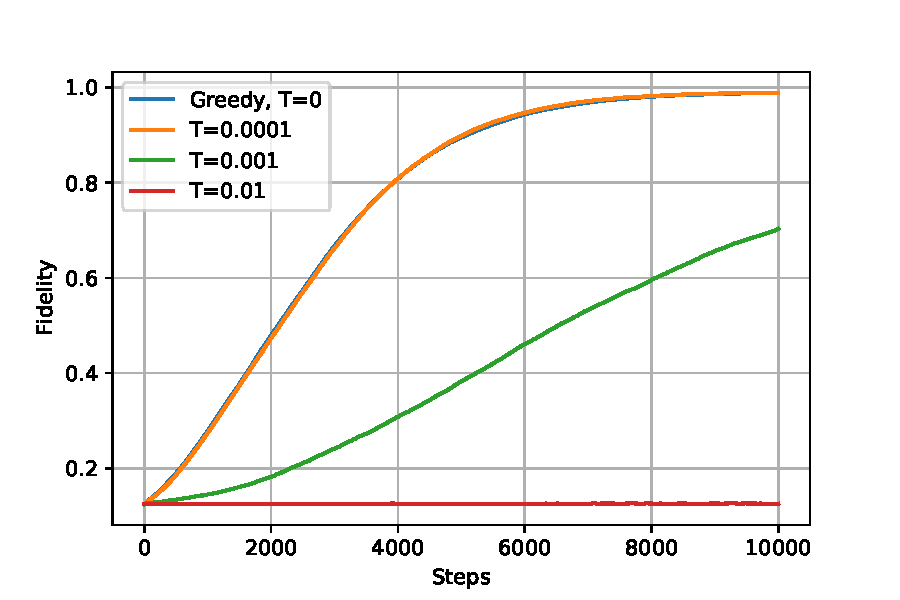
\includegraphics[width=.45\linewidth]{latex/figures/mcc_three_qubit_smallRot.pdf}   % this width should be half of the width of the other two images
    \caption{Three qubits, small rotations}
    \label{fig:sub-firstA}
\end{subfigure}
\caption{Small Rotations Basis on one, two and three qubits}\label{fig:smallRotMetropolis}
\end{figure}

In \autoref{fig:smallRotMetropolis}, we see Monte-Carlo compiling of one, two and three qubit random Haar unitaries (average of 100 random unitaries). The small rotations basis is used in all cases. In the one qubit case, it consists of the following gates: $\pm R_x, \pm R_y, \pm R_z$, where $\pm R_x$ is short for $R_x(\pm \frac{\pi}{128})$. This basis extends to two qubits by including all one-qubit rotations for both qubits, i.e. $R_j\otimes I$ and $I\otimes R_j$, in addition to all two-qubit rotations: $\pm XX, \pm YY, \pm ZZ$, where $\pm XX = \cos(\frac{\pi}{256})I\otimes I \mp i \sin(\frac{\pi}{256})X \otimes X$. The basis extends to three or more qubits in a similar way.\\

From \autoref{fig:smallRotMetropolis}, we see that the Monte-Carlo compiler was able to successfully compile the unitaries within the tolarence of $0.99$ in a reasonable number of steps: Roughly $1250$, $2500$ and $10000$ steps for one, two and three qubits. An interesting results is that the greedy approach ($T=0$) always outperformed the Metropolis approach ($T>0$) for any number of qubits. Any amount of explorations resulted in a poorer solution, which means that the most greedy approach is the optimal. In this sense, the small rotations basis makes the compiling of the unitaries seem like a \emph{convex} problem, which is very interesting. This might arise from the great flexibility of the small rotations, being able to rotate the state a small amount in any direction. For any given sequence of basis gates, $U_n$, it is possible to (pseudo-)continuously transform it into any other sequence $U_n'$ by changing one gate at a time without getting stuck in a local minima. This is exemplified in \autoref{fig:smallRot}.  


\begin{figure}[h]
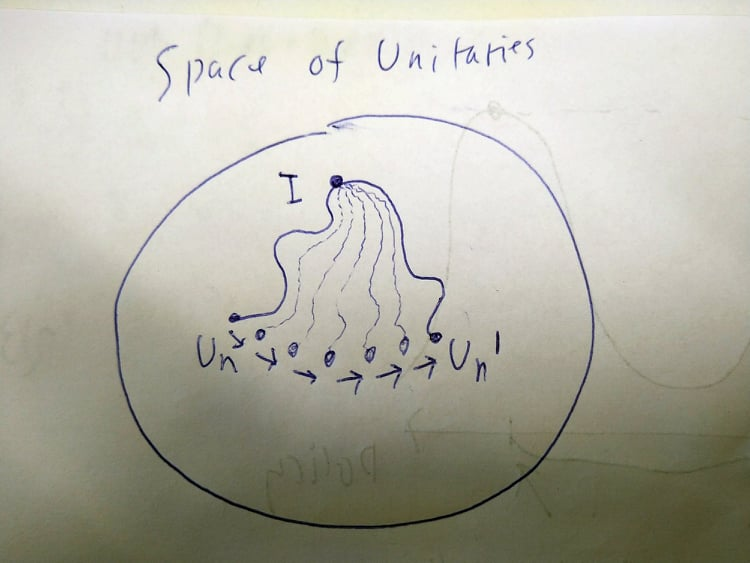
\includegraphics[width=8cm]{latex/figures/smallRot.jpg}
\caption{A sequence of small rotations being continuously transformed into another sequence of small rotations.}
\label{fig:smallRot}
\end{figure}
In the above figure, we see that one sequence of gates can be continuously transformed into another sequence by performing changes to one gate at a time. Thus, large jumps in the space of unitaries are not required, so there is no risk of getting stuck in local minima. This great flexibility, however comes at a big price: to account for all possible ways of rotating the state, the number of gates one needs to include for $n$ qubits can be expressed as 

\begin{equation}\label{eq:smallRot}
    N_n = 6\sum_{i=1}^{n}{{n}\choose{i}}.
\end{equation}
For example, we have $N_1 = 6, N_2 = 18, N_3 = 42, N_4 = 90$. This is a factorial increase, which makes it intractable to use for a high number of qubits. Further more, the small rotations basis set is not characteristic for the basis sets actually implemented on physical hardware. Even so, it could be useful as a benchmark for testing different (AI) compiling strategies because. Also, it is not clear if the basis set loses its convex nature if its size is constrained (e.g. its size is constrained to be scale polynomially by omitting some of the rotational directions).\\

\autoref{fig:HRCMetropolis} shows compiling of unitaires using the HRC basis set for one, two and three qubits. Unlike the small rotations basis set, HRC is highly non-convex in nature. To get out of local minima, $T>0$ is required, and higher temperatures usually yield better solutions. The Monte-Carlo compiler was not able to compile the unitaries within the tolerance 0.99 with HRC for the given hyperparameters, showing that it is indeed a much harder optimisation problem. While HRC is not implemented on real hardware, as same with small rotations, it is closer in nature to real implementations in the sense that it is highly discrete in nature and prone to getting stuck in local optima.



\begin{figure}[H]
\begin{subfigure}{.5\textwidth} 
    \centering
    % include first image
    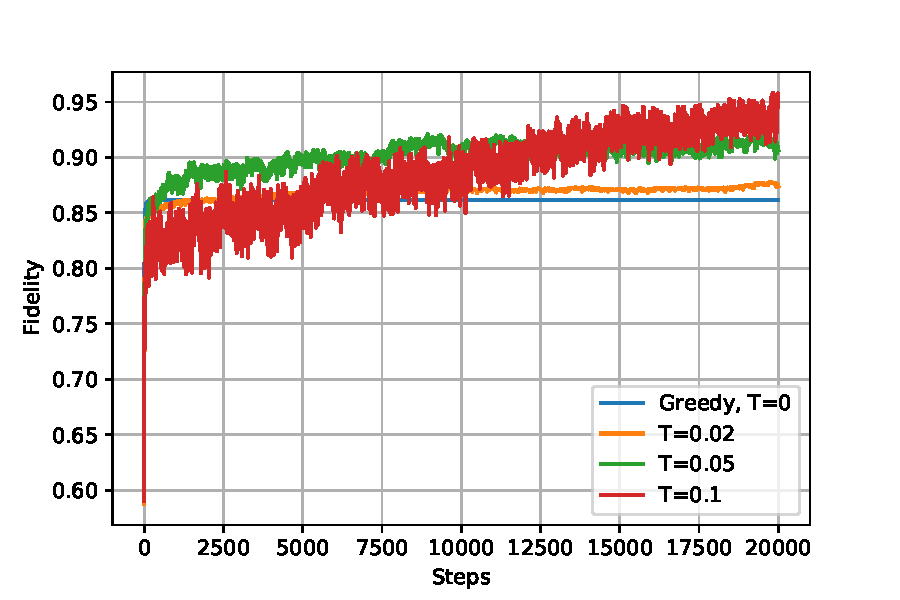
\includegraphics[width=.9\linewidth]{latex/figures/mcc_one_qubit_HRC.pdf}  % this sets the image to fill 90% of the available space -> 45% of the line width in total. 
    \caption{One qubit, HRC}
    \label{fig:sub-first}
\end{subfigure}
\begin{subfigure}{.5\textwidth}
    \centering
    % include second image
    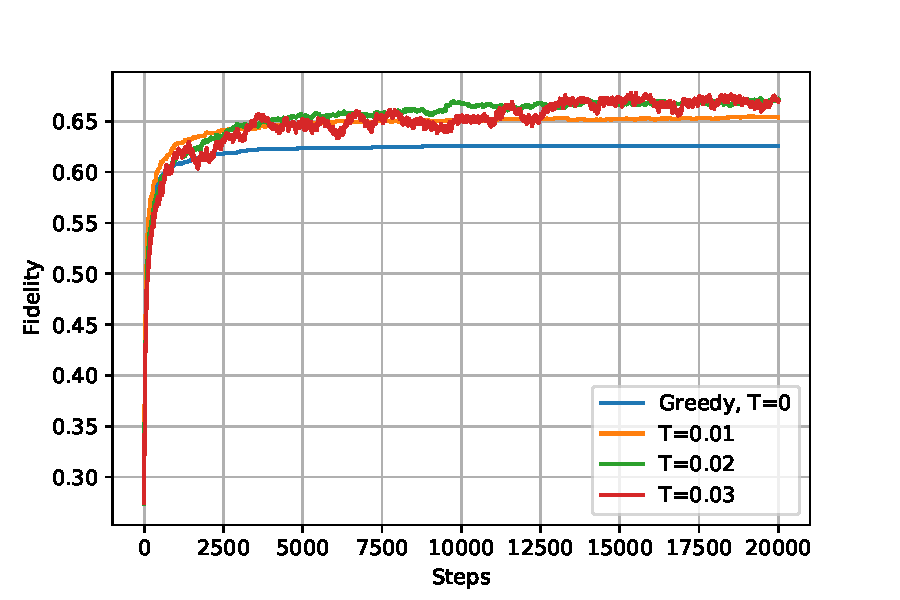
\includegraphics[width=.9\linewidth]{latex/figures/mcc_two_qubit_HRC.pdf}  
    \caption{Two qubits, HRC}
    \label{fig:sub-second}
\end{subfigure}


\begin{subfigure}{\textwidth}
    \centering
    % include first image
    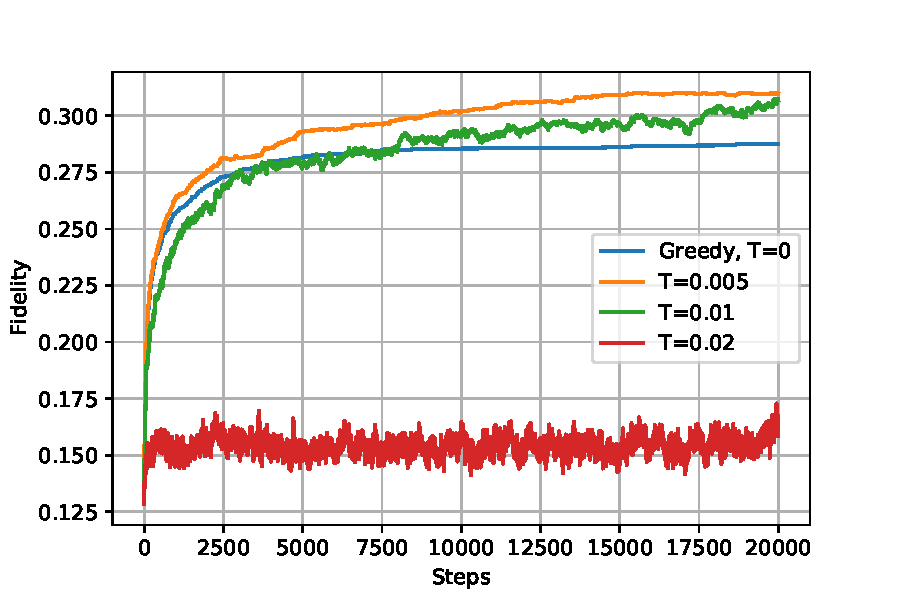
\includegraphics[width=.45\linewidth]{latex/figures/mcc_three_qubit_HRC.pdf}   % this width should be half of the width of the other two images
    \caption{Three qubits, HRC}
    \label{fig:sub-firstA}
\end{subfigure}
\caption{HRC Basis on one, two and three qubits}
\label{fig:HRCMetropolis}
\end{figure}

From the above figure, we see that non-zero $T$ is necessary for avoiding getting stuck in local minima when using the HRC basis set.

\subsubsection*{Results, Annealing Approach}









\newpage


\section{Ideas}

\subsection{Increase exploration for DQS agent by introducing a sparse reward function}

\cite{DQSRL} use a Reinforcement Learning agent for optimizing the parameters of a parameterized circuit using a learned policy. The resulting circuit should approximate a target state when applied to an initial state.
\newline
\newline
The agent seems to struggle with finding optimal parameters, as conventional optimization methods, such as gradient descent, are able to find much better parameters. This is likely a symptom of the agent's struggle to explore the space of possible policies. This can maybe be alleviated using a \emph{sparse} reward function. \cite{DQSRL} uses a reward function formulated as 

\[   
r_t = 
     \begin{cases}
       \text{0} &\quad\text{t $<$ n}\\
       \text{$f(|\psi_{Target}\rangle, |\psi_{DQS}\rangle)$} &\quad\text{t $=$ n}\\
     
     \end{cases},
\]
however, this type of reward is prone to getting stuck on local optima: Let's say the agent has discovered a policy that yields a reward(fidelity) $R=0.8$, and that there exists some other policy that yields $R=0.9$. Will the agent be able to discover this new policy? This can be difficult if the intermediate policies between the current policy and desired policy result in a much lower reward. The agent will thus avoid exploring these intermediate policies (since they offer a lower reward), and it will fail in discovering the much better policy (see the figure under).

\begin{figure}[h]
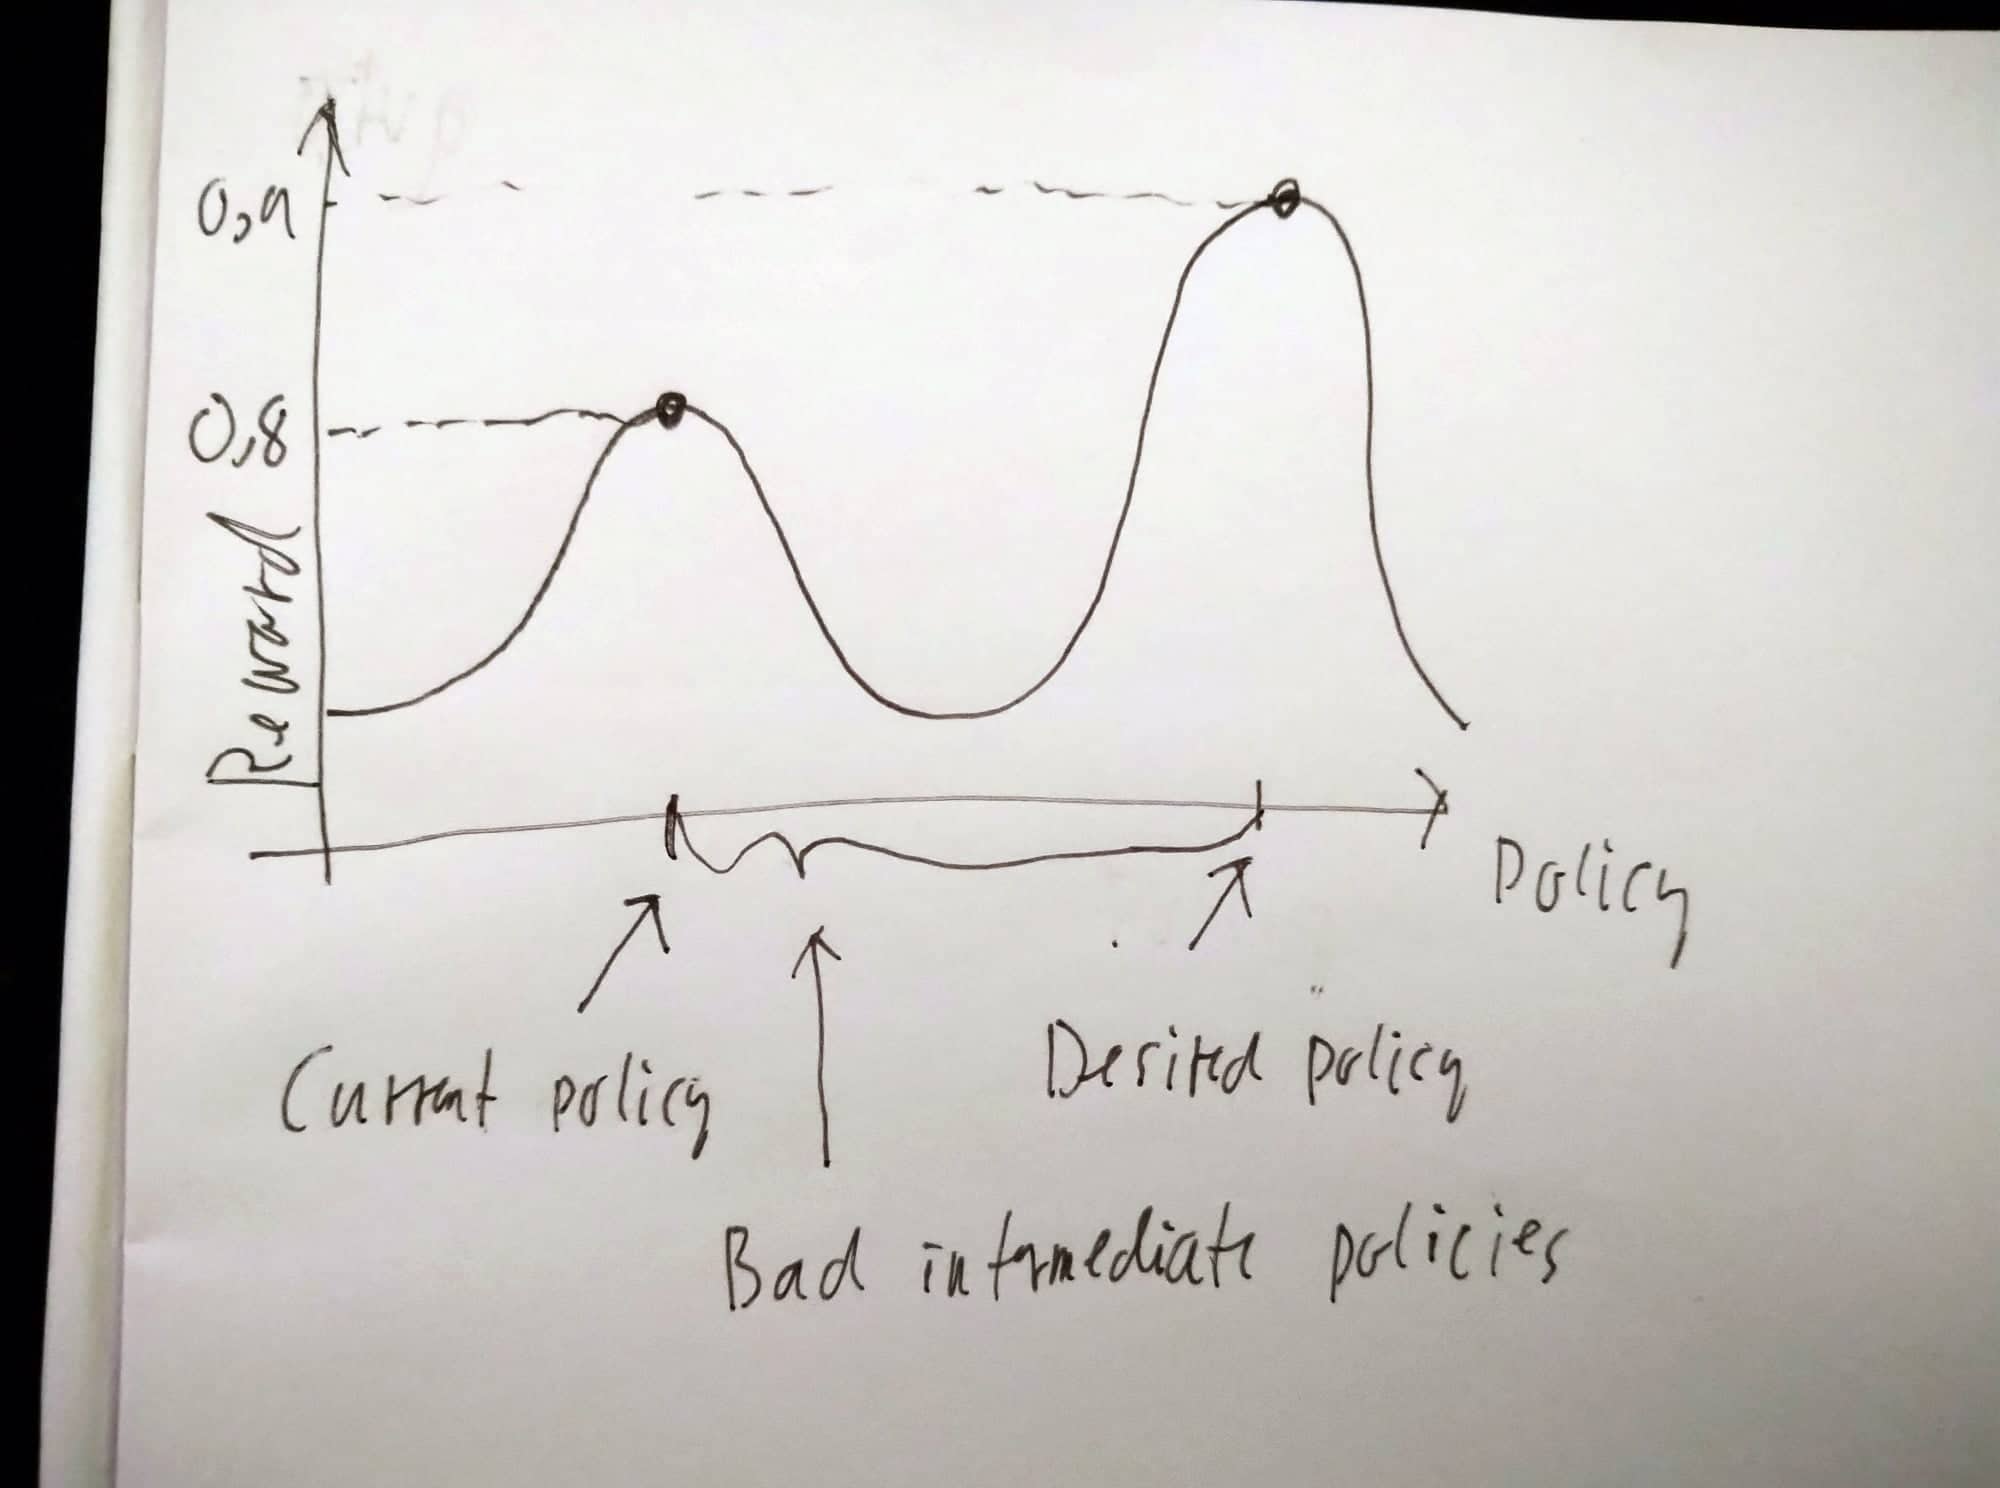
\includegraphics[width=8cm]{policy.png}
\end{figure}
\\
Drawing inspiration from \cite{QuantumComp}, we can introduce a sparse reward function

\[   
r_t = 
     \begin{cases}
       \text{0} &\quad\text{$f(|\psi_{Target}\rangle, |\psi_{DQS}\rangle)>0.9$}\\
       \text{$-1$} &\quad\text{otherwise}\\
     
     \end{cases},
\]
This reward function is binary, giving the agent only a reward (in this case, a reward of zero, which is relativly better than minus one) if it discovers a policy that yields a fidelity of 0.9 (or better), which we wanted. A sparse reward does not suffer from the problem of getting stuck on local optima, since it is only rewarded for finding policies which actually solve the problems to the desired accuracy. In this sense, the the agents gets to explore a larger space of policies. Of course, this comes with a tradeoff. For all episodes where the agent does not find a solution, it gets a constant reward of $-1$ for each action. This is uninformative, and can not help "guide" the agent towards better solutions. This can lead to slower training. However, there are techniques to help the agent also learn from episodes where it failed, such as Hindsight Experience Replay (HER) \cite{andrychowicz2018hindsight, QuantumComp}. 
\newline
\newline
I have a working Python framework that can implement HER and sparse reward functions.

\subsection{Hybrid Action Space}

Both \cite{QuantumComp} and \cite{DQSRL} utilize Reinforcement Learning to sequentially build a quantum circuit using elementary building blocks. The resulting circuit should approximates some target, either a target unitary or a target state(when applied to some initial state), respectively. Both methods can be though of as quantum compiling.  
\newline
\newline
\cite{QuantumComp} and \cite{DQSRL} use, respectively, a discrete and a continuous set of elementary building blocks. The former use finite sets of elementary quantum gates, for example the HRC set:

\begin{align*}
    V_1 = 
    \frac{1}{\sqrt{5}}
    \begin{bmatrix}
    1 & 2i\\
    2i & 1
\end{bmatrix}\\
V_2 = 
\frac{1}{\sqrt{5}}
\begin{bmatrix}
    1 & 2\\
    -2 & 1
\end{bmatrix}\\
V_3 = 
\frac{1}{\sqrt{5}}
\begin{bmatrix}
    1 +2i & 0\\
    0 & 1 - 2i
\end{bmatrix}
\end{align*}
The latter use a parameterized layer of trapped ion gates on the form
\begin{equation}\label{eq:layer}
    U_t = U^{xx}(\theta^{xx}_t)\prod_{j}{U^{z}(\theta^{z,j}_t)U^{x}(\theta^{x,j}_t)},
\end{equation}
defined by a vector of continuous parameters. In both scenarios, the agent must pick the best sequence of elementary building blocks to reconstruct the target. The action space of the agents is therefore, respectively, discrete and continuous. A possible extension of either(or both) works is to generalize the agents to a hybrid action space, allowing for a set of mixed discrete and continuous actions. There are two reasons to do this:
\subsubsection*{Reason One}
For \cite{QuantumComp}, a hybrid action space allows for sets of basis gates often implemented on real quantum computers. The HRC basis set, while efficient for theoretical calculations, is not implemented on real quantum computers in practice. This is also true for other sets of basis gates, like Clifford+T or discrete Pauli rotations. Many of IBM quantum computers implement the following gates\cite{j2020quantum}:

\begin{equation*}
    B = \{U_1(\lambda), R_X(\pi/2), CNOT\},
\end{equation*}
where

\begin{equation*}
    U_1(\lambda) = 
    \begin{bmatrix}
    1 & 0\\
    0 & e^{i\lambda}
    \end{bmatrix}
\end{equation*}
and $\lambda$ is a continuous parameter. Thus, this is a both discrete and continuous set, requiring a hybrid action space. This is also true for the set of gates SpinQ can implement.  

\subsubsection*{Reason Two}
For \cite{DQSRL}, a hybrid actions space could allow for building circuits where each layer has varying structure. Instead of constraining the structure to follow \ref{eq:layer}, the set of elementary building blocks could be generalized to 

\begin{equation*}
    B = \{U^{XX}(\theta), U^Z(\theta), U^X(\theta)\},
\end{equation*}
allowing for arbitrary combination of the gates (e.g. two $U^{XX}$ gates in a row). This increased flexibility could improve the method of \cite{DQSRL} (perhaps only marginally, since the main problem is not to find the best structure of the layers, but the best parameters $\theta$ of the gates.) 
\newline
\newline
The implementation of agents with hybrid action spaces is a well-known problem in the AI community \cite{xiong2018parametrized}, with existing literature.  
\newpage

\section{Notes on Papers}

\begin{equation}
    a = \sum_{i=3}^{10} i^2
\end{equation}

This was found in \cite{sack2022avoiding}


Figure retrieved from "Quantum Compiling with\newline
Deep Reinforcement Learning" (Moro et. al. 2021) 



\bibliographystyle{alpha}
\bibliography{sample}

\end{document}